% This is a (brief) model paper using the achemso class
% The document class accepts keyval options, which should include
% the target journal and optionally the manuscript type.

\documentclass[journal=langd5, manuscript=article, layout=twocolumn]{achemso}

% Place any additional packages needed here.  Only include packages
% which are essential, to avoid problems later. Do NOT use any
% packages which require e-TeX (for example etoolbox): the e-TeX
% extensions are not currently available on the ACS conversion
% servers.

\usepackage[version=3]{mhchem} % Formula subscripts using \ce{}
\usepackage[T1]{fontenc}       % Use modern font encodings
\usepackage{amsmath, amssymb, amsfonts}
\usepackage{graphicx, gensymb}

% If issues arise when submitting your manuscript, you may want to
% un-comment the next line.  This provides information on the
% version of every file you have used.
%\listfiles

% Place any additional macros here.  Please use \newcommand* where
% possible, and avoid layout-changing macros (which are not used
% when typesetting).

\SectionNumbersOn
\graphicspath{ {Figures/} }
\newcommand{\tdc}[3][]{\frac{\mathrm{d}^{#1}#2}{\mathrm{d}#3^{#1}}} % total differential change.
\newcommand{\pdc}[3][]{\frac{\partial^{#1} #2}{\partial #3^{#1}}} % partial differential change.
\newcommand{\td}[1]{\mathrm{d}#1}
\newcommand{\pd}[1]{\partial#1}

% Meta-data block
% ---------------
% Each author should be given as a separate \author command.
%
% Corresponding authors should have an e-mail given after the author
% name as an \email command. Phone and fax numbers can be given
% using \phone and \fax, respectively; this information is optional.
% The affiliation of authors is given after the authors; each
% \affiliation command applies to all preceding authors not already
% assigned an affiliation.
%
% The affiliation takes an option argument for the short name.  This
% will typically be something like "University of Somewhere".
% The \altaffiliation macro should be used for new address, etc.
% On the other hand, \alsoaffiliation is used on a per author basis
% when authors are associated with multiple institutions.

\author{V. S. Akella}
\affiliation{Collective Interactions Unit, OIST Graduate University, Okinawa, Japan 904-0495}
\author{D. K. Singh}
\affiliation{Collective Interactions Unit, OIST Graduate University, Okinawa, Japan 904-0495}
\author{R. K. Singh}
\affiliation{School of Engineering, Brown University, 182 Hope Street, Providence, RI 02906, USA}
\author{S. Mandre}
\affiliation{School of Engineering, Brown University, 182 Hope Street, Providence, RI 02906, USA}
\email{shreyas_mandre@brown.edu}
\author{M. M. Bandi}
\affiliation{Collective Interactions Unit, OIST Graduate University, Okinawa, Japan 904-0495}
\email{bandi@oist.jp}

% The document title should be given as usual. Some journals require
% a running title from the author: this should be supplied as an
% optional argument to \title.

\title[]{Dynamics of a Camphoric Acid boat at the air-water interface} 

% Some journals require a list of abbreviations or keywords to be
% supplied. These should be set up here, and will be printed after
% the title and author information, if needed.

\abbreviations{CA, DI}
\keywords{Marangoni flow, Self-propulsion}

% The manuscript does not need to include \maketitle, which is
% executed automatically.

\begin{document}

% The "tocentry" environment can be used to create an entry for the
% graphical table of contents. It is given here as some journals
% require that it is printed as part of the abstract page. It will
% be automatically moved as appropriate.

% \begin{tocentry}

% Some journals require a graphical entry for the Table of Contents.
% This should be laid out ``print ready'' so that the sizing of the
% text is correct.

% Inside the \texttt{tocentry} environment, the font used is Helvetica
% 8\,pt, as required by \emph{Journal of the American Chemical
% Society}.

% The surrounding frame is 9\,cm by 3.5\,cm, which is the maximum
% permitted for  \emph{Journal of the American Chemical Society}
% graphical table of content entries. The box will not resize if the
% content is too big: instead it will overflow the edge of the box.

% This box and the associated title will always be printed on a
% separate page at the end of the document.

% \end{tocentry}

% The abstract environment will automatically gobble the contents
% if an abstract is not used by the target journal.

\begin{abstract}
We experimentally study the physics of camphoric acid loaded agarose gel tablets (cboats) at the air-water interface. Camphoric acid spreads over the air-water interface due to the interfacial tension forces. When a cboat is held fixed at the air-water interface, the spread radius grows as power law in time with a scaling exponent of $\frac{1}{2}$, in agreement with observed scaling for the time-dependent spread radius for volatile substances\cite{troian1998} at the air-water interface. As the camphoric acid spreads, shear stresses caused by the Marangoni forces lead to the development of boundary layer at the air-water interface. Scaling analysis using boundary layer approximation suggests that the fluid velocity in the boundary layer scales as a power law in distance with a scaling exponent of $-\frac{3}{5}$. When let go, a cboat is spontaneously set in motion by the interfacial tension gradients. We explain the cboat dynamics in terms of a dimensionless quantity $\xi = \frac{\Delta\sigma\ a}{\rho\ u^{2}\ a^{2}}$, where $\Delta\sigma\ a$ is the interfacial tension force acting along a characteristic length $a$ of cboat; $\rho\ u^{2}\ a^{2}$ is the drag force experienced by the cboat. By definition, $\xi = 1$ when the interfacial tension force and drag force are equal and the cboat moves with terminal velocity. Through control of interfacial tension, we show three distinct modes, viz. harmonic, steady, and periodic cboat motion arise for $\xi > 1$, $\xi \sim 1$ and $\xi < 1$ respectively.    
\end{abstract}

% Start the main part of the manuscript here.

\section{Introduction}
The scientific interest in the motion of objects governed by the interfacial tension gradients started with Alessandro Volta\cite{volta1787} who was studying the motion of camphor fragments on the surface of water. However, Van der Mensbrugghe\cite{mensbrugghe1869} first explained that the motion is due to the decrease in surface tension of water by the camphor fragments. Further, Tomlinson\cite{tomlinson1869} and Rayleigh\cite{rayleigh1889} studied the motion of camphor fragments on the surface of water in detail. Since then many researchers have been studying motion of objects driven by the interfacial tension gradients. These studies are at Reynolds numbers spanning over 4-5 orders of magnitude ($\sim 10^{-3} - 10^{2}$). Few examples are: motion of liquid droplets on a solid surface with surface energy gradient\cite{whitesides1992}, motion of ethanol driven gel tablets on the air-water interface\cite{velev2012}, propulsion of Belousov-Zhabotinsky drops in flourinated oil\cite{herminghaus2011}, motion of camphor boats at the air-water interface\cite{nakata2001}. The object's motion shows distinct modes when the interfacial tension is modified. In the current work, we attempt to explain these modes of motion using a ratio of the relevant forces involved in motion viz. interfacial tension force and drag force. Moreover, we experimentally demonstrate these modes in the motion of camphoric acid boats at the air-water interface. 

\section{Experimental Section}
Hot agarose solution (5\% weight-to-volume) in de-ionized (DI) water (Milli-Q Integral Water Purification System with resistivity, $\rho=18.2\ \mathrm{M}\Omega\cdot\mathrm{cm}$ at 25\celsius) was placed between two glass plates, set 1 mm apart with aluminum spacers, to obtain gel sheets of uniform thickness 1 mm, upon cooling. Gel tablets of 3 mm diameter were cut out from the sheet with a punch (3 mm diameter Biopunch, Ted Pella Inc.). These gel tablets were introduced in camphoric acid (CA) (Wako Pure Chemical Industries, Ltd., Cat. No. 036-01002) saturated methanol solution and left for 2 hours for CA to diffuse into the gel tablets. Prior to experiments, gel tablets were rinsed in DI water to precipitate CA in the gel matrix; henceforth these gel tablets are referred to as cboats. The experimental study consists of characterizing the stationary and moving cboat at the air-water interface. We describe the basic experimental methods for each study in the following sections. 
\subsection{Stationary Cboat}
\begin{figure}[ht]
    \begin{center}
       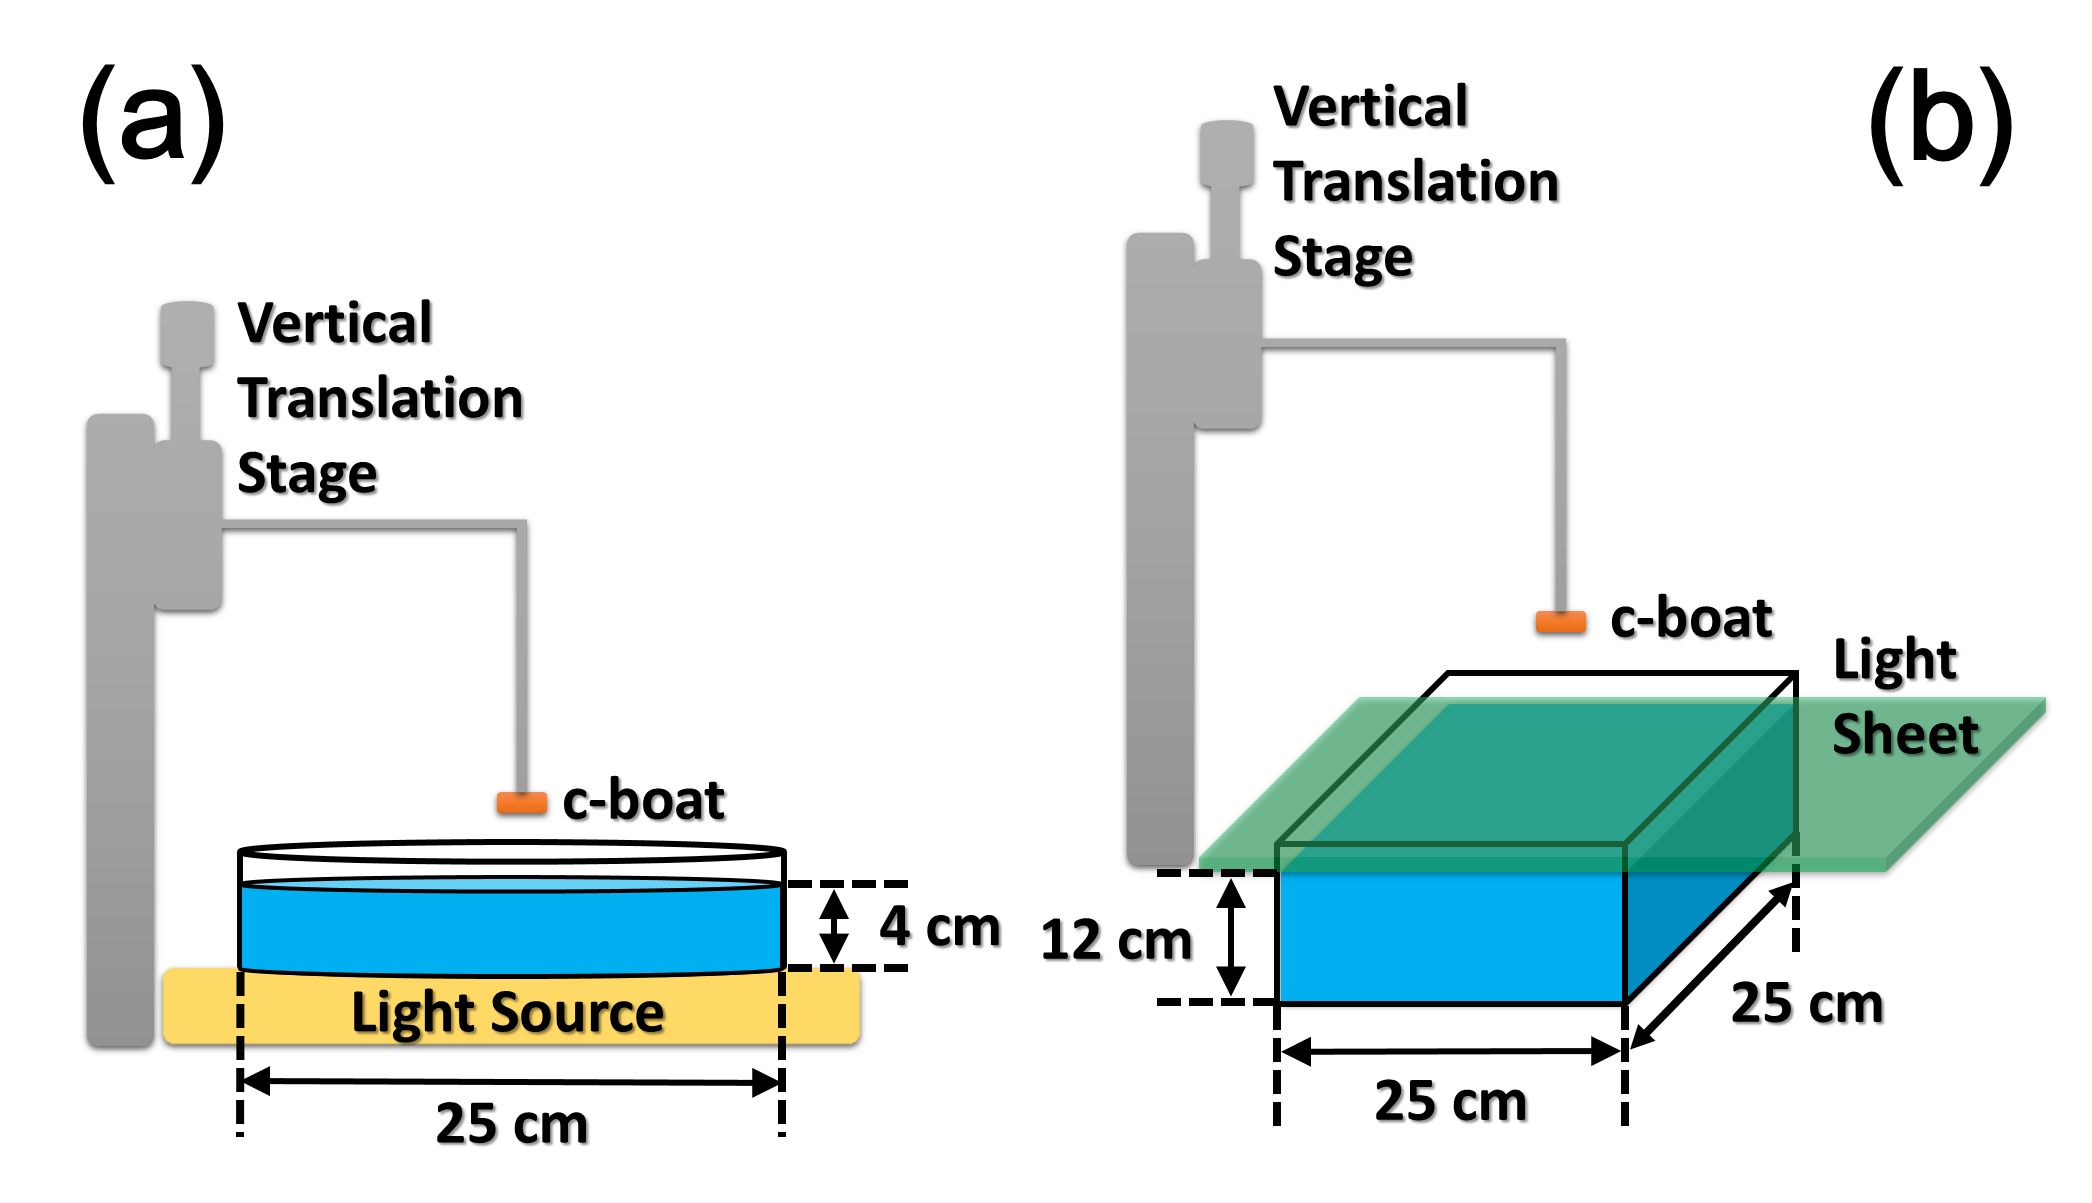
\includegraphics[scale=0.25]{figure1.png}
    \end{center}
    \caption{Experimental set up for the stationary cboat experiments.}
    \label{fig:expsetup}
\end{figure}
The experimental setup (figure~\ref{fig:expsetup}) consists of (1) a glass container filled with DI water (2) an L-shaped steel wire with one end firmly attached to a vertical translation stage (3) an illumination source and (4) Phantom v641 hi-speed camera, located directly above the glass container. The cboat is attached at the free-end of the steel wire. At the beginning of the experiment the steel-wire-arrangement is lowered using the tranlational stage such that the cboat makes a gentle contact with the air-water interface and for the rest of the experiment the cboat is left un-disturbed. For the transient regime experiments (figure~\ref{fig:expsetup}a), we used a 25 $\mathrm{cm}$ diameter and 5 $\mathrm{cm}$ height glass petri dish filled with approximately 2 liters of DI water and the petri dish is illuminated using a light tablet from bottom. To visualize the spread dynamics, the air-water interface is covered with hydrophilic tracer particles ($d = 50\ \mu \mathrm{m}$, specific gravity = 0.25) at low packing fractions, $\phi \leq 0.2$. We did \emph{not} observe any effect of tracer particles on the spread dynamics at packing fractions, $\phi \leq 0.2$. The spread dynmics are recorded at 1000 frames per second with 100 $\mu \mathrm{s}$ exposure time using the hi-speed camera. 
\begin{figure*}[ht]
    \centering
	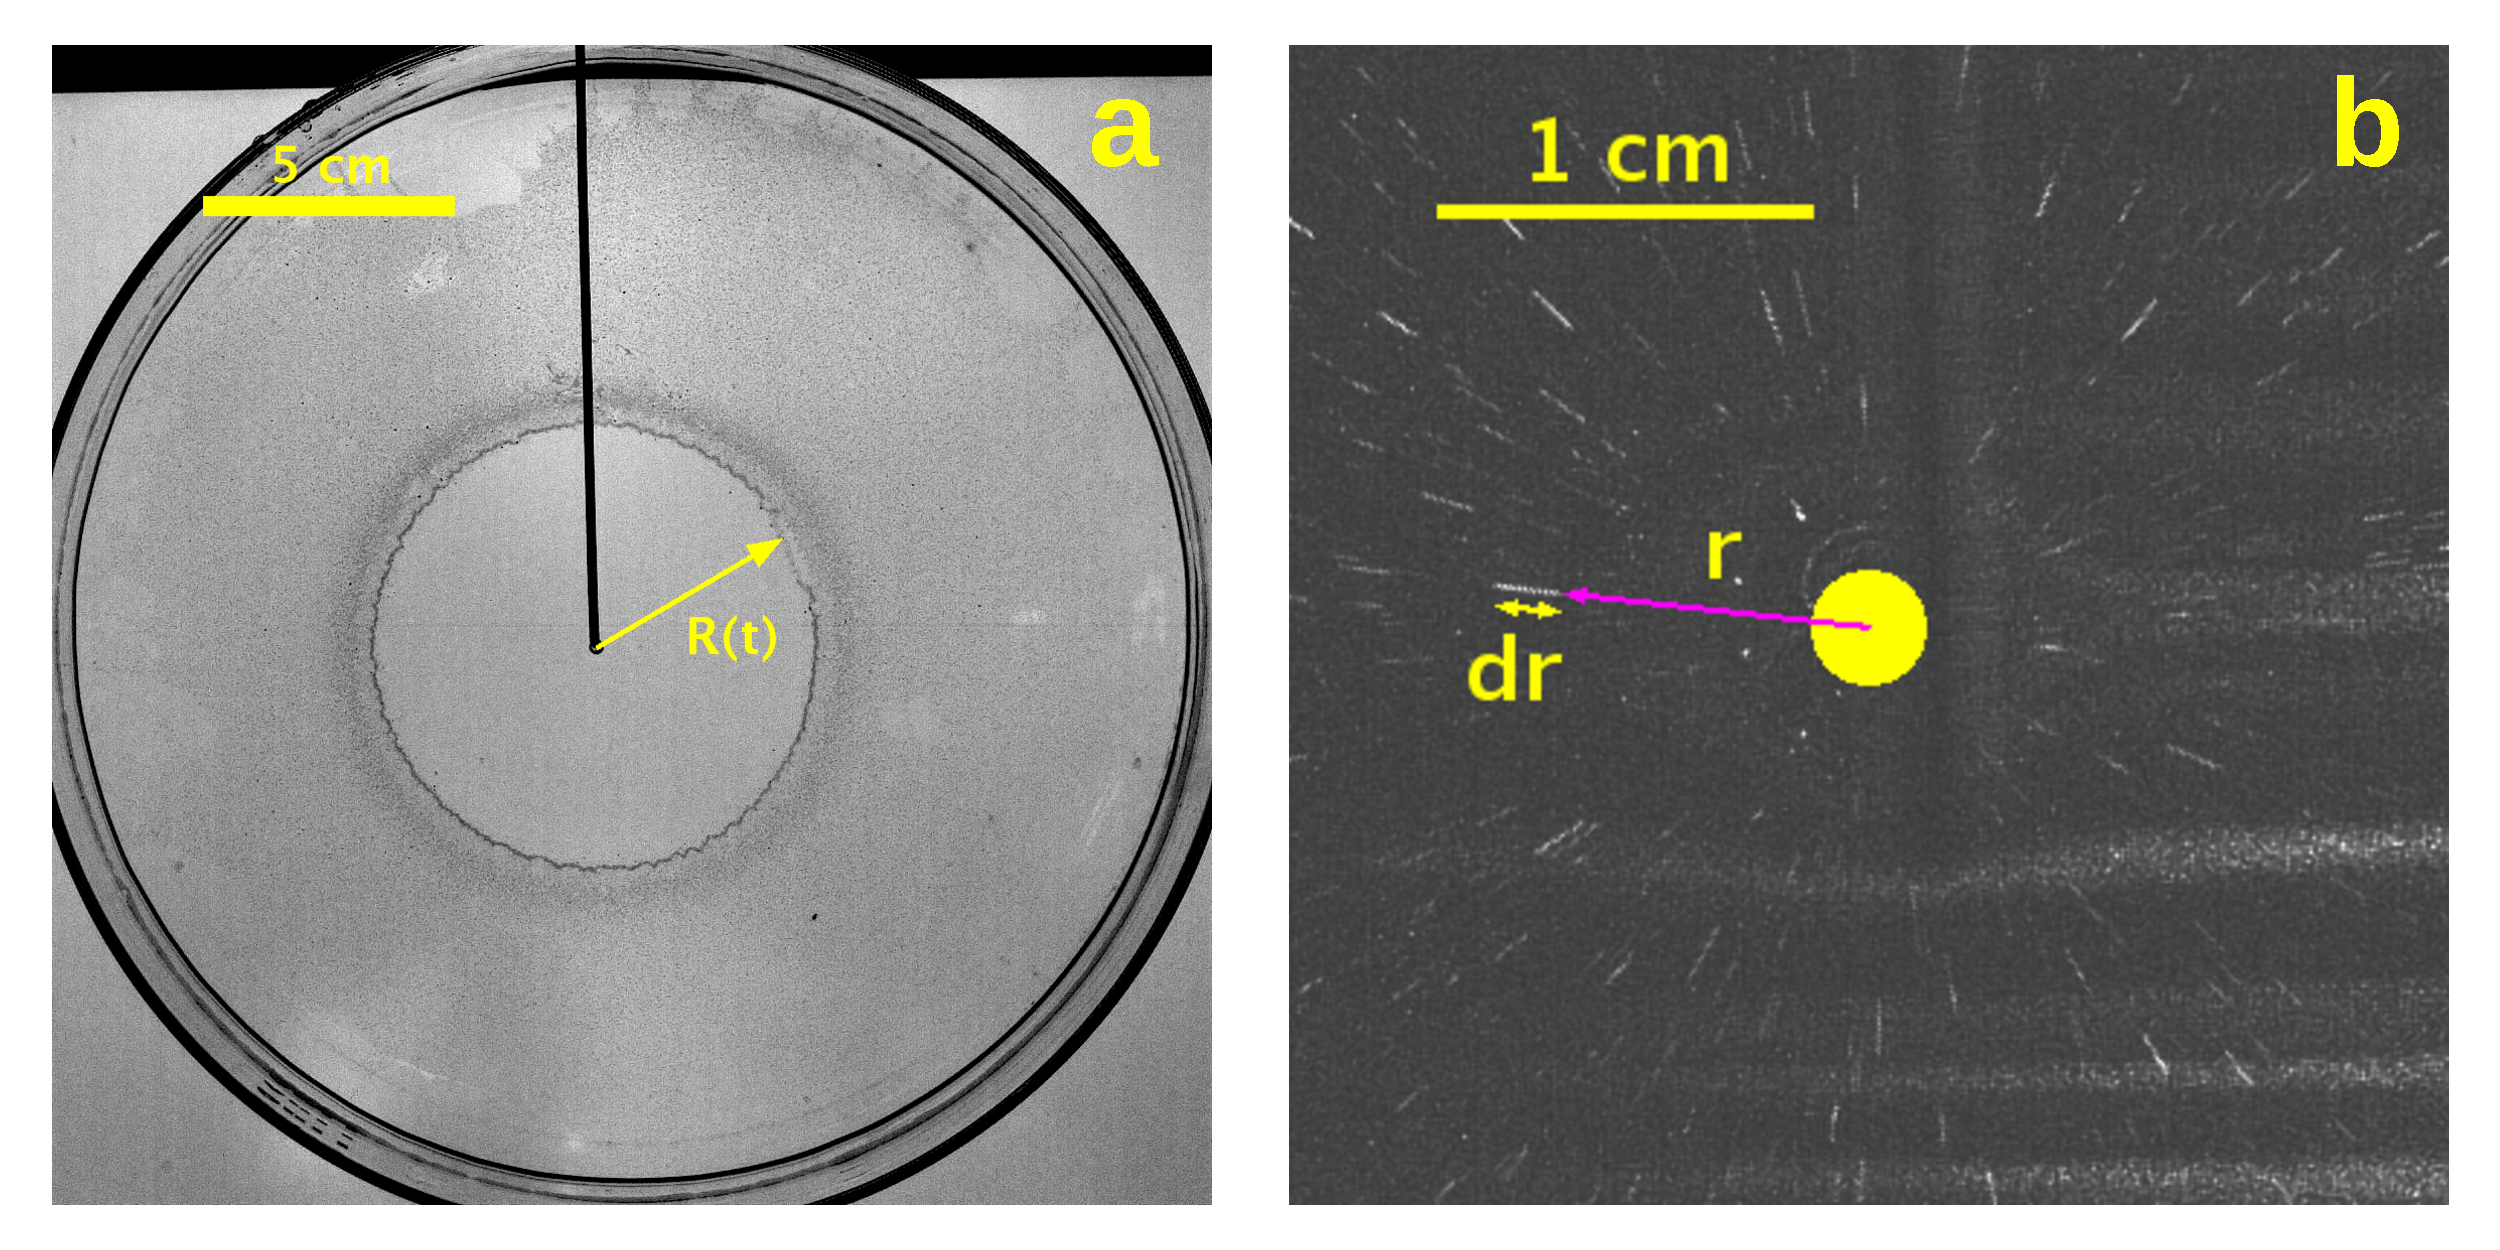
\includegraphics[width=\textwidth]{figure2.pdf}	

	\caption{(a) Caphoric acid spread radius at an instant in time, visualized using hydrophilic tracer particles. (b) Measurement of radial velocity at a distance $r$ from the center of the cboat. The length of the streak, $\td{r}$ is the distance traveled by the tracer particle in time $\td{t} = 0.1\ \mathrm{sec}$ }
	\label{fig:statboat}
\end{figure*}
As CA spreads over the interface, the tracer particles are pushed away radially outwards creating a particle-free zone. The radius of the particle-free zone is measured (using ImageJ) manually from a time series of images. Figure~\ref{fig:statboat}a shows the particle-free zone at an instant in time. For the steady state regime experiments (figure~\ref{fig:expsetup}b), we used a glass container of dimensions 25 $\mathrm{cm}$ $\times$ 25 $\mathrm{cm}$ $\times$ 25 $\mathrm{cm}$ filled with approximately 8 liters of DI water and the air-water interface is illuminated with a laser sheet of thickness $\approx$ 3 $\mathrm{mm}$ such that the bulk layers are minimally illuminated. The fluid velocity at the interface is measured by mixing un-measurably small quantity of neutrally buoyant tracer particles ($d < 10\ \mu\mathrm{m}$). The motion of the tracer particles is recorded at 300 frames per second with 1 $\mathrm{ms}$ exposure time using the hi-speed camera. Figure~\ref{fig:statboat}b is a resultant image obtained by adding 30 such consecutive frames. The lengths of the streaks are manually measured (using ImageJ). The length of the streak, $\td{r}$ (figure~\ref{fig:statboat}b) is the distance in centimeters (converted to centimeters using appropriate pixel to centimeter conversion factor) traveled by the tracer particle in $\td{t}=$ 0.1 $\mathrm{sec}$ at a radial distance $r$ (figure~\ref{fig:statboat}b) from the center of the cboat. 
\subsection{Moving Cboat}
The basic experimental setup consisted of a 25 $\mathrm{cm}$ diameter glass petri dish filled to a height of 4 cm ($\approx$ 2 liters) with DI water and placed atop an LED light tablet. A cboat was gently placed at the air-water interface and its motion was recorded from above using a Nikon D800E camera at 30 frames per second. The cboat positions and velocities were calculated using image analysis programs written inhouse. The position and velocity calculations are confined to a region $3.6\ \mathrm{cm}$ away from the wall of the petri dish to eliminate any influence of the boundary on the cboat dynamics. The choice of $3.6\ \mathrm{cm}$ is based on the experimental result (discussed in section~\ref{sec:steady}) that at a radial distance $3.6\ \mathrm{cm}$ measured from the center of the cboat the CA concentration reduces to zero due to dissolution of CA in water. Using published tables \cite{mysels1986}, we introduced metered dosage of Sodium Dodecyl Sulfate (SDS) (Wako Pure Chemical Industries, Ltd., Cat. No. 196-08675) to modify the air-water interfacial tension when necessary. We independently confirmed the actual surface tension values using the pendant drop method (OneAttension Theta tensiometer) at 25\celsius.

\section{Results and Discussion}
\subsection{Stationary Cboat}
\label{sec:statboat}
Camphoric acid is a mildly surface active compound which decreases the air-water interfacial tension through dissolution. When a cboat is placed at the air-water interface, interfacial forces cause CA molecules to spread over the surface. This spreading cannot continue indefinitely due to dissolution of CA in water. As a result, radially symmetric CA concentration gradients (surface tension gradients) are set up around the cboat out to a finite distance. Owing to the slower dissolution kinetics of camphoric acid compared to the spread dynamics, the concentration front reaches a farther distance than the steady state distance which is the distance, measured from the center of the cboat, at which the convection flux and the dissolution flux of CA balance each other. As a result, the concetration front retraces to the steady state distance (see movie S1 in the supplementary information). Note that, the hydrophilic tracer particles trace back because by spreading they minimize the interfacial energy of air-water interface\cite{nudurupati2009}. For brevity, we discuss our findings in two parts, 1. The transient regime and 2. The steady state regime. 
\subsubsection{Transient Regime}
\label{sec:transient}
The transient regime is observed from the instance of cboat's contact with the air-water interface to the time when the CA spread radius reaches a steady state value. During the transient regime, we observe two spreading stages (1) the divergent stage: during which the CA molecules are drawn out of the cboat and spread radially outwards over the interface soon after the cboat's contact with the air-water interface (2) the convergent stage: during which the spread radius shrinks to the steady state value due to dissolution of CA in water. The spread radius, measured during the divergent stage, follows a power law in time with a scaling exponent of $\frac{1}{2}$ (figure~\ref{fig:caspread}) which is in agreement with the observed scaling for the spread of volatile oils\cite{troian1998} at the air-water interface. The identical scaling behavior for the spread of CA and volatile oils at the air-water interface suggests that the system needs a pathway for the loss of material from the air-water interface either through dissolution, evaporation or both. Note that, when there is no dissolution/evaporation the spread dynamics \emph{never} reach a steady state, as observed in the case of spreading of non-volatile oils at the air-water interface\cite{jensen1995, mahadevan2011}, for which the spread radius scales with time as $t^{3/4}$. Figure~\ref{fig:caspread} is a plot of the spread radius $R(t)$ as a function of time measured during divergent stage. Note that, as dissolution dominates the spread radius plateaus at later times however in figure~\ref{fig:caspread} those data are not included. We attribute the scatter in the data around the fit to the experimental variation in the depth of cboat sitting below the air-water interface from trial to trial.   
\begin{figure}[ht]
    \begin{center}
       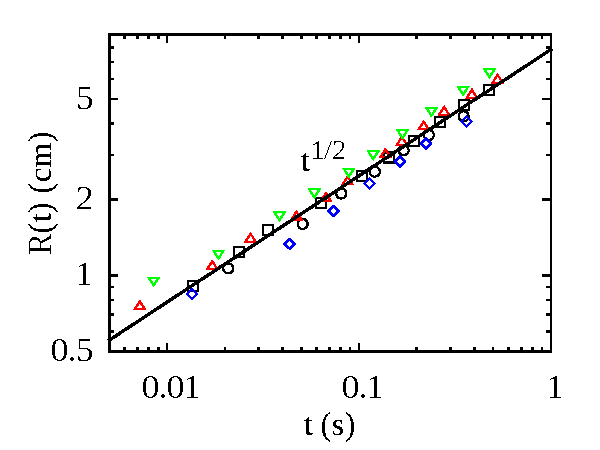
\includegraphics[width=\linewidth]{rvst_transient.pdf}
    \end{center}
    \caption{Camphoric acid radial spread vs. time. The radial front is visualized using 50 $\mu m$ hydrophilic tracer particles sparsely sprinkled at the air-water interface. Symbols correspond to different experimental trials.}
    \label{fig:caspread}
\end{figure}
\subsubsection{Steady State Regime}
\label{sec:steady}
The spread of CA over the air-water interface reaches a steady state when the convection (diffusion + advection) flux equals the dissolution flux. As a result, steady state CA concentration gradients are setup out to a finite distance around the cboat which in turn lead to the interfacial tension gradients and are the source of solutal Marangoni forces. The Marangoni forces shear the air-water interface resulting in radially symmetric flow around the cboat. Note that, the radial distance, measured from the center of cboat, at which the flux balance is achieved happens to be smaller than the maximum spread distance measured in the divergent stage (explained in section~\ref{sec:transient}) because of slower dissolution kinetics than the spread dynamics. We derived (Appendix~\ref{app:uvsr}) a power law scaling for the fluid velocity as a function of radial distance at the air-water interface with a scaling exponent of $-\frac{3}{5}$. Figure~\ref{fig:radvel} shows the experimentally measured interfacial radial velocity as a function of radial distance and the fit to the proposed scaling. The large scatter in velocity data is attributed to the erroneous measurement of $\td{r}$, which is the distance traveled by a tracer particle in a given time $\td{t}$ (figure~\ref{fig:statboat}b). The tracer particles, which are neutrally buoyant, go in and out of plane of measurement during the fluid flow and as a result $\td{r}$ measurements are inaccurate.
\begin{figure}[ht] 
    \begin{center}
       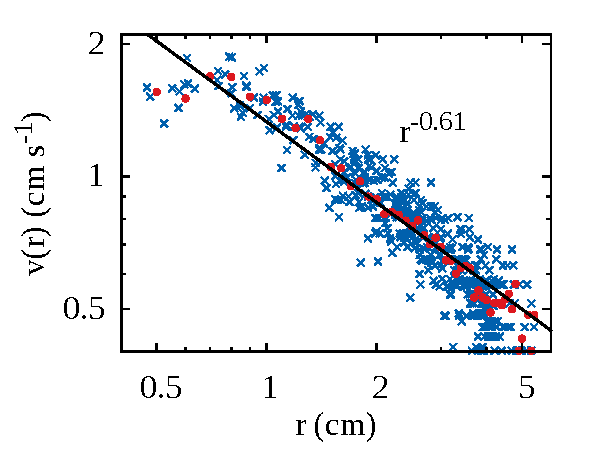
\includegraphics[width=\linewidth]{urvsr_steady.pdf}
    \end{center}
    \caption{Radial velocity measured at the air-water interface for a stationary cboat.}
    \label{fig:radvel}
\end{figure}
% =======================================================================
\subsection{Moving Cboat}
\subsubsection{Mechanism of self-propulsion}
\label{sec:propmech}
When a cboat is placed at the air-water interface, radially symmetric interfacial tension gradients are set up around the cboat as explained in section~\ref{sec:steady}. Ambient fluctuations spontaneously break this symmetry and sharpen the gradients leading to a net force acting on the cboat. When let go, the cboat is set in motion by these interfacial tension gradients. The boat's motion ensures the asymmetry is amplified and maintained thereby permitting its continued motion. Owing to constant dissolution, the cboat motion continues until it exhausts all CA molecules. Whereas dissolution does globally reduce the surface tension of water, a single boat never contains sufficient CA ($\sim 7\ \mathrm{mg}$) to achieve this; surface tension of CA saturated water ($\sim 8\ \mathrm{g\ l^{-1}}$) is $\sim 60\ \mathrm{dy\ cm^{-1}}$. Over the course of an experiment, water replaces CA removed from the boat starting at the periphery and progressively proceeds radially inwards. Consequently, CA concentration at the cboat edge constantly decreases resulting in weaker interfacial tension gradients which decrease the boat speed as time progresses (figure~\ref{fig:lifetime}); this bears upon results to follow and will be discussed later. Assuming first order rate kinetics \cite{atkins2014} for the dissolution of camphoric acid in water, we fit the cboat speed as a function of time to an exponential decay with the decay constant, $\tau \sim 35\ \mathrm{min}$; $\tau$ therefore represents the cboat life time. Whereas a cboat could also lose CA via evaporation/sublimation, it is negligible relative to dissolution.

\begin{figure}[ht]
    \begin{center}
       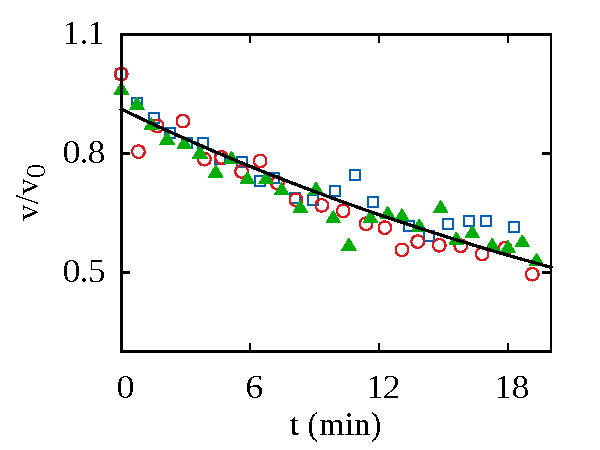
\includegraphics[width=\linewidth]{lifetime.pdf}
    \end{center}
    \caption{Normalized Cboat speed vs. time, fit to $\mathrm{e}^{-\frac{t}{\tau}}$ where $\tau$ represents the life time of a cboat. Symbols correspond to different experimental trials.}
    \label{fig:lifetime}
\end{figure}

\subsubsection{Oscillatory Motion of the cboat}
\label{sec:oscboat}
\begin{figure*}[ht]
	\centering
	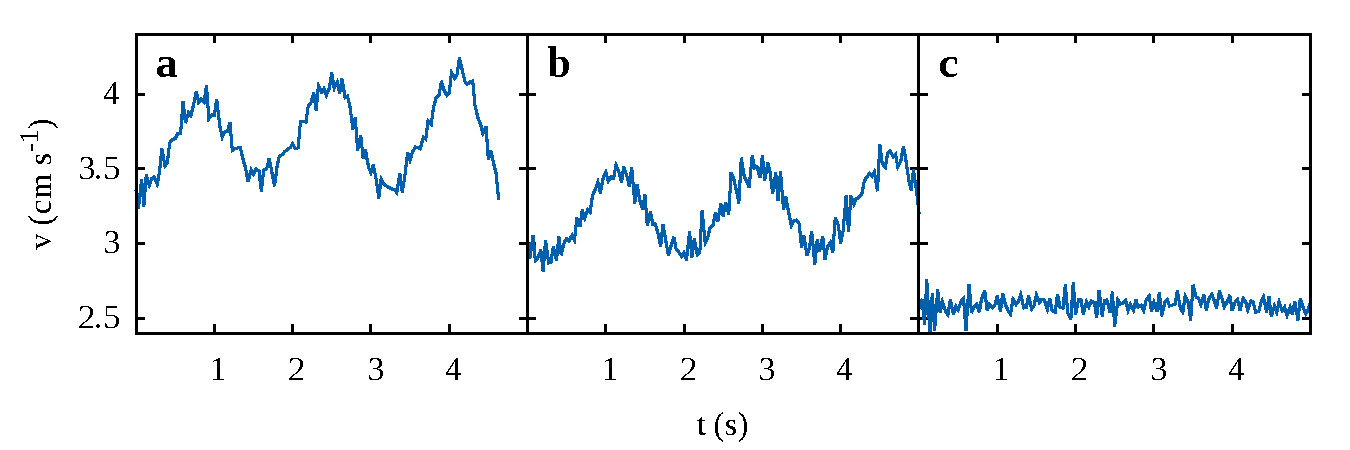
\includegraphics[width=\textwidth]{uvst_72dypcm.pdf}
	\caption{{\bf (a)} at $\sim 4\ \mathrm{min}$, {\bf (b)} at $\sim 7\ \mathrm{min}$, {\bf (c)} at $\sim 16\ \mathrm{min}$}
\label{fig:uvst_72dypcm}
\end{figure*}
Besides the continuous decrease in speed, the cboat also exhibits oscillatory dynamics on a shorter time scale (few seconds) compared to the life time (approximately an hour) of the cboat. Figure~\ref{fig:uvst_72dypcm} shows the time traces of the cboat speed at different intervals during the course of experiment. The average speed at different intervals decreases due to the dissolution of CA in water as mentioned in previous section. The oscillations arise due to the competition between the Marangoni force and the drag force. The Marangoni force accelerates the cboat to a larger speed $u$, however the drag force, which scales as $u^{2}$ (explanation follows), decelerates the cboat. As the cboat slows down, the Marangoni force again acclerates the cboat. This driving and damping cycle leads to oscillations in cboat speed. When there is a balance between the driving and damping forces the cboat moves with terminal velocity, as shown in figure~\ref{fig:uvst_72dypcm}c. The amplitude of oscillations decreases and the period of oscillations increases (shown in figure~\ref{fig:uvst_65dypcm}) due to the dissolution of CA. In following section, we introduce a dimensionless quantity $\xi = \frac{\Delta\sigma\ a}{\rho\ u^{2} a^{2}}$ in order to qualitatively describe the oscillatory dynamics of cboat. Furthermore, the value of $\xi$ was experimentally varied by changing the air-water interfacial tension using SDS.

The interfacial tension force, $\mathbf{F}_{\sigma}$ and the drag force $\mathbf{F}_{D}$ are given by,
\begin{equation}\label{eq:allfgeneral}
\begin{aligned}
\mathbf{F}_{\sigma} &= \oint_{C} \sigma \ \hat{\mathbf{n}} \ \td{l} \\
\mathbf{F}_{D} &\sim \rho\ a^{2} \left|\mathbf{u}\right|^{2} \hat{\mathbf{u}}
\end{aligned}
\end{equation}
where, $\mathbf{F}_{D}$ is the viscous drag acting on the cboat and $a$ is the diameter of cboat. Note that, the cboat motion is \emph{not} in Stoke's regime ($\mathbf{F}_{D} \propto \mathbf{u}$) where the inertial forces are negligible in comparison to viscous forces ($\mathit{Re} << 1)$. In case of the cboat system $\mathit{Re} \sim 100$. The contour integral apperaing in equation~\ref{eq:allfgeneral} is evaluated along a circular contour $C$ (figure~\ref{fig:schematic}a), whose center is at the center of the cboat, and the resultant is the force acting on the cboat due to the interfacial tenion gradients. Obviously, the value of the integral is zero when surface tension gradients are symmetric. 
\begin{figure}[ht]
    \centering
	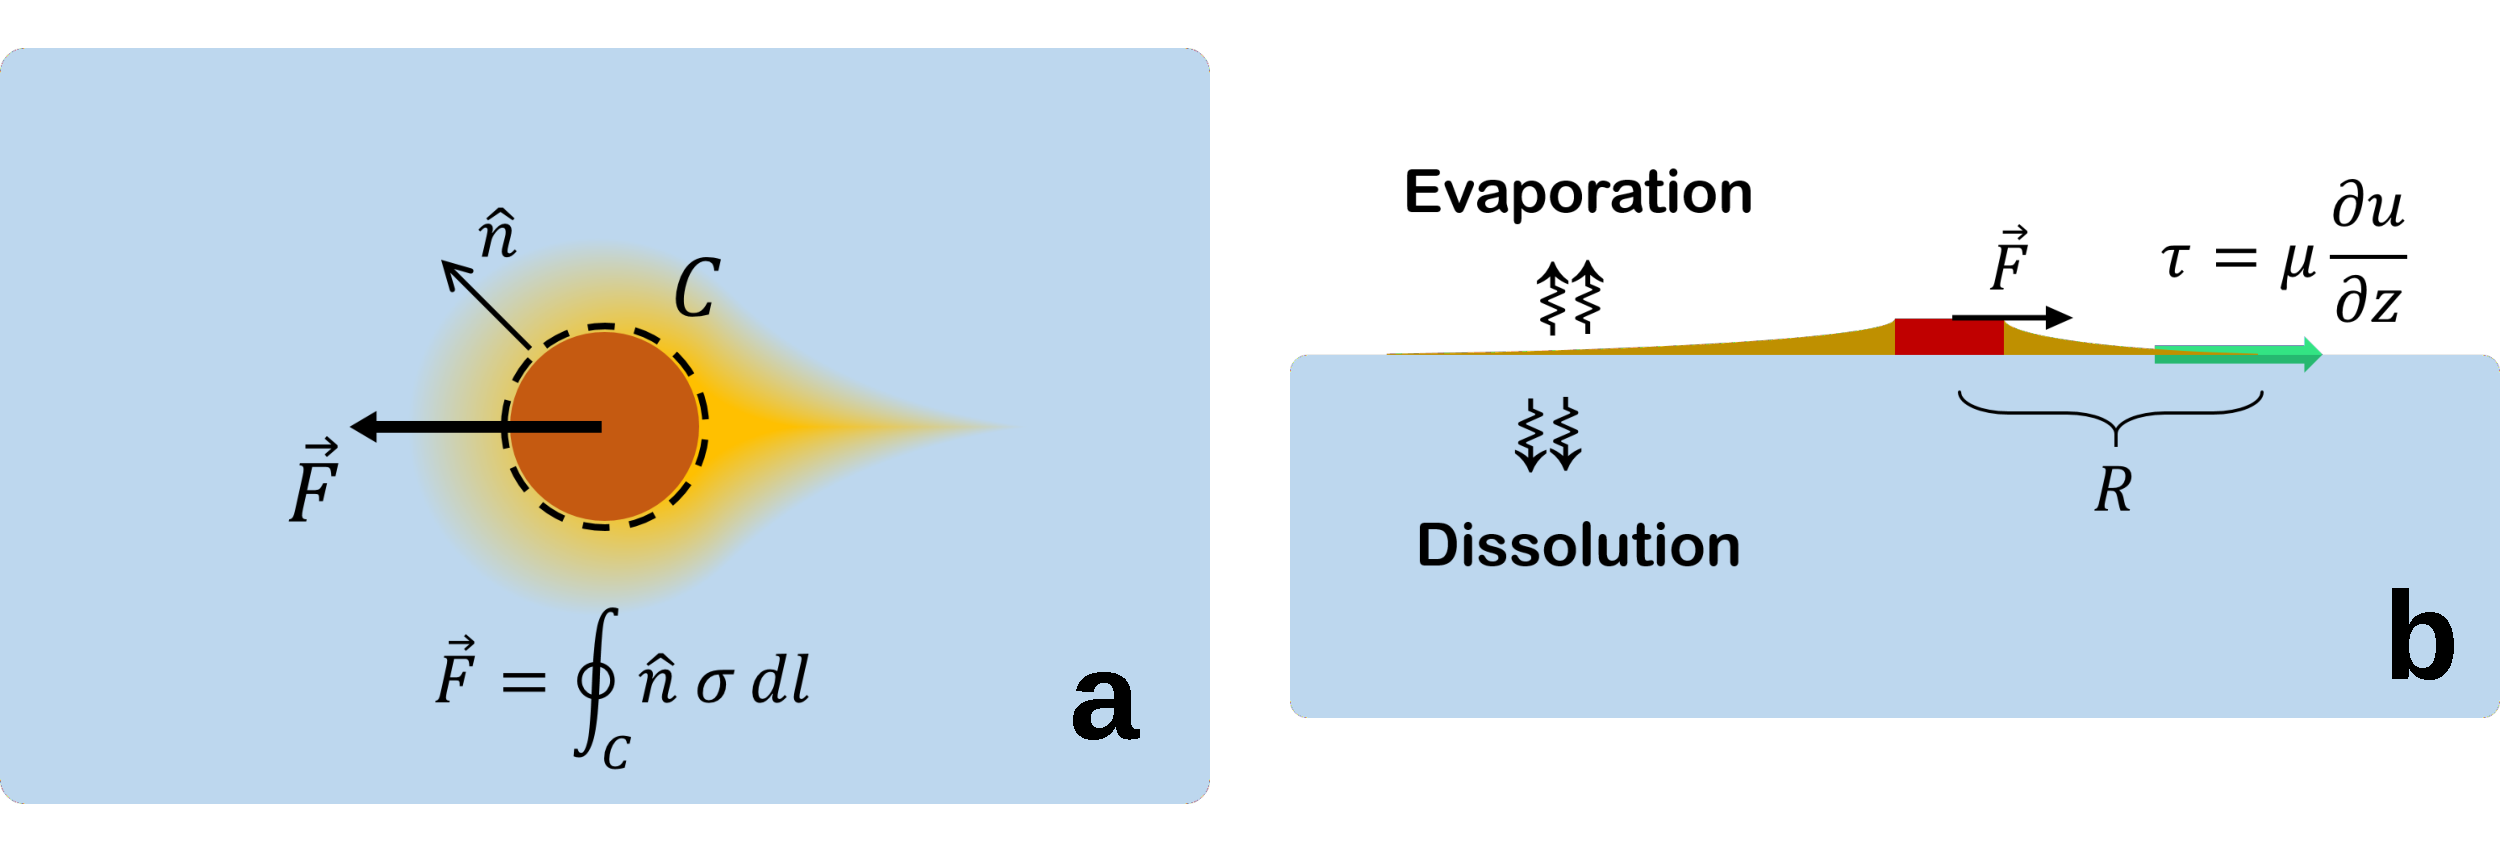
\includegraphics[width=\linewidth]{figure4.pdf}
	\caption{Schematic of cboat in motion (a) top view (b) side view obtained along a horizontal line bisecting the cboat and along the direction of motion. Viscous drag \emph{not} shown in schematic. In case of CA, evaporation/sublimation is negligible in comparison to dissolution.}\label{fig:schematic}
\end{figure}

For brevity, let us assume that the cboat exhibits rectilinear motion then the set of equations~\ref{eq:allfgeneral} simplifies to
\begin{equation}\label{eq:allfsimple}
\begin{aligned}
F_{\sigma} &\sim \Delta\sigma\ a \\
F_{D} &\sim \rho\ u^{2}\ a^{2}
\end{aligned}
\end{equation}
where, $\Delta\sigma\ a$ is the interfacial tension force acting along a length $a$ and $\rho\ u^{2}\ a^{2}$ is the drag force acting on the cboat.
\paragraph{Dimensionless Quantity, $\xi$}
The dimensionless quantity $\xi$ is defined as,
\begin{equation}
\xi = \frac{\text{interfacial force}}{\text{drag force}} = \frac{\Delta\sigma\ a}{\rho\ u^{2}\ a^{2}}
\end{equation}
Note that, the choice of drag force $F_{D} = \rho\ u^{2}\ a^{2}$ is appropriate for the case of cboat but the definition of $\xi$ as ratio of driving and damping forces is in general applicable to various systems. When the interfacial and drag forces are equal the cboat moves with terminal velocity and $\xi = 1$ (figure~\ref{fig:uvst_72dypcm}c).
\begin{figure*}[ht]
	\centering
	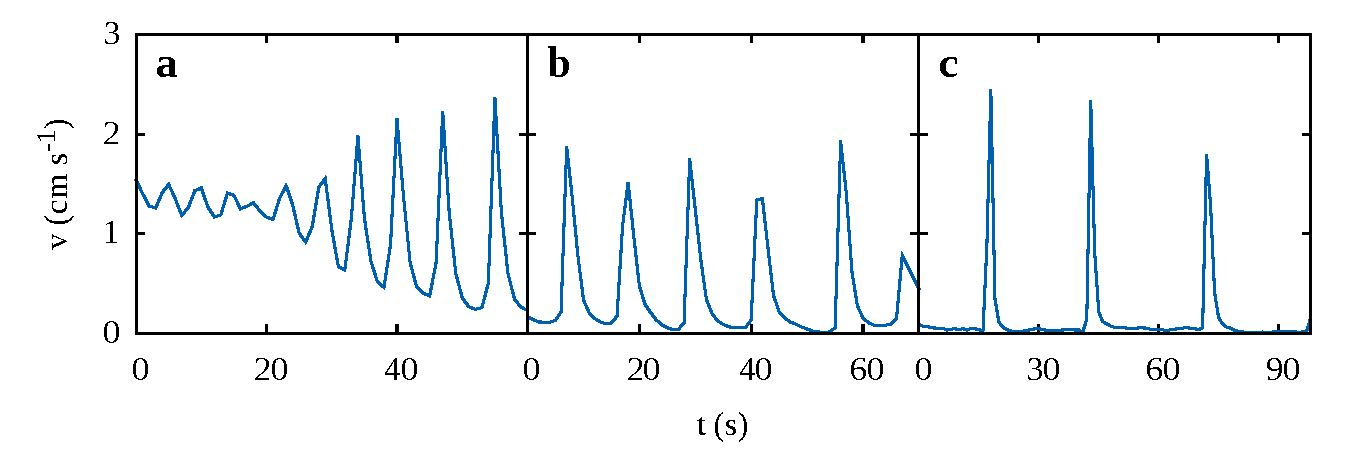
\includegraphics[width=\textwidth]{uvst_65dypcm.pdf}
	\caption{{\bf (a)} at $ 0\ \mathrm{min}$, {\bf (b)} at $\sim 7\ \mathrm{min}$, {\bf (c)} at $\sim 15\ \mathrm{min}$}
\label{fig:uvst_65dypcm}
\end{figure*}

Naturally, the dimensionless quantity $\xi$ constantly decreases during the experiment due to the dissolution of CA in water. However, we varied $\xi$ by modifying the air-water interfacial tension using SDS. Figure~\ref{fig:uvst_65dypcm} shows the speed traces of a cboat at different intervals of time when the air-water interfacial tension is lowered to $65\ \mathrm{dy\cdot cm^{-1}}$. We observe that, the average speed of the cboat at different intervals decreases and the period of the oscillations increases. Another subtle observation is the distance travelled by the cboat, area under the speed vs. time curves, between oscillations is approximately equals to the distance, $R$ out to which CA molecules are spread by the Marangoni flow and beyond $R$, CA concentration is zero due to dissolution. During the course of experiment $R$ constantly decreases due to dissolution of CA in water. 
\begin{figure}[ht] 
    \centering
       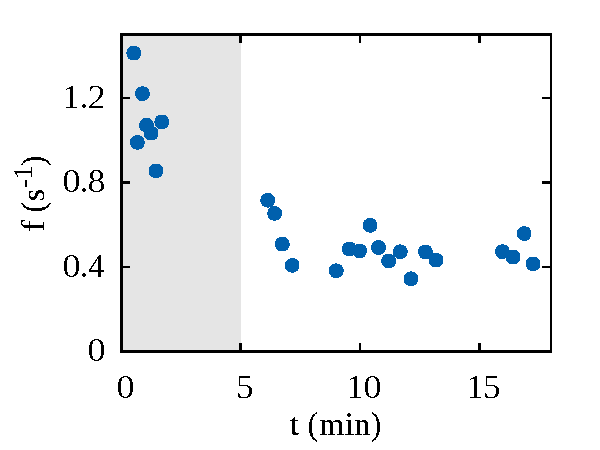
\includegraphics[width=\linewidth]{freqvst.pdf}
    \caption{Frequency of oscillation vs. time. Grayed out area is the transient phase during which excess CA present on the surface of the cboat.}
    \label{fig:freqvst}
\end{figure}
The period of oscillation is governed by the advection time scale, $\tau_{A} \sim \frac{R}{U_{M}}$, which is the time taken by a CA molecule to get advected from the periphery of the cboat to a distance $R$ and $U_{M}$ is the Marangoni flow velocity. When $\sigma = 72\ \mathrm{dy\cdot cm^{-1}}$, the period of oscillation is $\sim 2\ \mathrm{sec}$ (figure~\ref{fig:uvst_72dypcm}a) and from stationary boat experiments in section~\ref{sec:steady} the radial velocity measured at the air-water interface is $U_{M} \sim 1.5\ \mathrm{cm\ s^{-1}}$ with the steady state spread radius $R \sim 3\ \mathrm{cm}$, which yields the advection time scale $\sim 2\ \mathrm{sec}$ which is in aggrement with the period of oscillation. Note that, when $\sigma = 65\ \mathrm{dy\cdot cm^{-1}}$ the radial velocity measurements are extremely sensitive to ambient fluctuations as these velocities are very small. The technique used for the measurements reported in figure~\ref{fig:radvel} does not achieve the level of sensitivity needed to measure the velocities at $\sigma = 65\ \mathrm{dy\cdot cm^{-1}}$. Figure~\ref{fig:freqvst} shows the frequency of oscillation $f = \frac{2\pi}{\tau_{A}}$ during the course of the experiment performed at $\sigma = 65\ \mathrm{dy\cdot cm^{-1}}$. The grayed out region is the transient phase which is a result of quick dissolution of CA particles which are loosely adhered to the surface of cboat i.e. which are not embedded in the gel matrix. Past the transient phase, frequency of oscillation constantly decreases due to dissolution of CA in water. Since the cboat is mostly not moving (figure~\ref{fig:uvst_65dypcm}) during the course of the experiment the dissolution rate is solely limited by diffusion of CA molecules in water which considerably increases the life time of cboat in comparison to a constantly moving cboat (figure~\ref{fig:uvst_72dypcm}). As a result we don't observe considerable change in the frequency during the course of the experiment. When the air-water interfacial tension is decreased to such an extent below which dissolution of CA in water has \emph{no} effect on the air-water interfacial tension results in \emph{no} motion of cboat. Figure~\ref{fig:uvst_sigma} shows the plots of cboat speed versus time at different air-water interfacial tensions. As shown in figure~\ref{fig:uvst_sigma}c, when $\sigma = 59\ \mathrm{dy/cm}$, cboat's motion ceases; note that the obseved non-zero speed is due to the drift of cboat because of ambient fluctuations.
\begin{figure*}[ht]
	\centering
	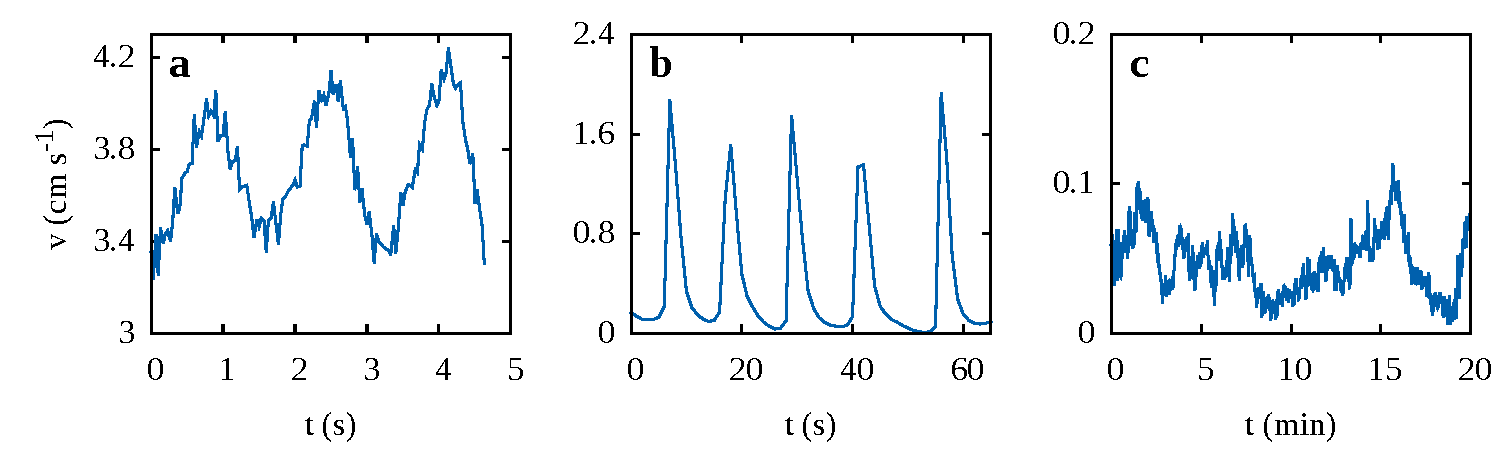
\includegraphics[width=\textwidth]{uvst_sigma.pdf}
	\caption{{\bf (a)} at $\sigma = 72\ \mathrm{dy\ cm^{-1}}$, {\bf (b)} at $\sigma = 65\ \mathrm{dy\ cm^{-1}}$, {\bf (c)} at $\sigma = 59\ \mathrm{dy\ cm^{-1}}$}
\label{fig:uvst_sigma}
\end{figure*}

\section{Summary}
\label{sec:summary}
When a cboat is held fixed at the air-water interface, camphoric acid (CA) molecules are drawn on to the air-water interface and spread radially outwards over the interface to minimize the air-water interfacial energy. The spread radius follows a $t^{1/2}$ power law scaling in time and is in agreement with observations on non-volatile oils\cite{troian1998}. The spread of CA reaches a steady state when there is a balance between the convection and dissolution of CA. The dissolved CA molecules modify the air-water interfacial tension. These interfacial tension gradients shear the air-water interface causing the underlying fluid to flow, known as solutal Marangoni flow. We derived a scaling law for the radial velocity of the shear flow at the air-water interface as function of radial distance by invoking the boundary layer approximation. The derived scaling law is: $v(r) \propto r^{-3/5}$ where $v(r)$ is the radial velocity at the interface and $r$ is the radial distance measured from the center of the cboat. Moreover, we experimentally confirmed that the radial velocity indeed agrees with the proposed scaling law as a function of radial distance. When let go, a cboat is spontaneously set in motion by the interfacial tension gradients. The cboat speed continuously decreases with time due to the dissolution of CA in water. We fitted the cboat speed to an exponential decay in time to obtain the life time of the cboat $\tau \sim 35\ \mathrm{min}$. Furthermore, we observed oscillations in the cboat speed at shorter time scales than the life time of the cboat. These oscillations occur as a result of competition between the driving (interfacial tension) forces and damping (drag) forces. We described the oscillations using a dimensionless quantity $\xi = \frac{\Delta\sigma\ a}{\rho\ u^{2}\ a^{2}}$ which quantifies the relative strengths of the forces involved in the system. When the forces are of equal strength $\xi = 1$ and the cboat moves with terminal velocity. We varied $\xi$ by changing the air-water interfacial tension using SDS. The oscillation frequency is governed by the advection time scale $\tau_{A} \sim \frac{R}{U_{M}}$, which is the time required for a CA molecule to be advected by the Marangoni flow, with a characteristic velocity $U_{M}$, to a characteristic distance $R$.

\begin{acknowledgement}
VSA, DKS, and MMB were supported by the Collective Interactions Unit at the Okinawa Institute of Science and Technology. MMB acknowledges L. Mahadevan for introducing the camphor boat system and subsequent scientific discussions, and D. Vu Anh for help with preliminary experiments. VSA would like to thank Pinaki Chakraborty for discussions. The authors acknowledge Kenneth J. Meacham III for help with experiments.
\end{acknowledgement}

% \begin{suppinfo}

% This will usually read something like: ``Experimental procedures and
% characterization data for all new compounds. The class will
% automatically add a sentence pointing to the information on-line:

% \end{suppinfo}

% The appropriate \bibliography command should be placed here.
% Notice that the class file automatically sets \bibliographystyle
% and also names the section correctly.

\bibliography{CBoat}
\newpage
\appendix
\numberwithin{equation}{section}
\section{Radial velocity at the air-water interface}
\label{app:uvsr}
Assumptions:
\begin{enumerate}
\item Amount of camphoric acid dissolved in water is negligible compared to the amount at the air-water interface.
\item There exists a boundary layer at the air-water interface due to the fluid flow driven by the interfacial tension gradients.
\item Air-water interfacial tension varies linearly with the concentration of camphoric acid.
\end{enumerate}
Let $c(r)$ and $u(r)$ be the radial concentration and velocity profiles at the air-water interface. 
Then the flux of camphor $q$ at a radial distance $r$ is: 
\begin{equation*}
q \sim r u_{r} c \implies c \sim \frac{q}{ru_{r}} 
\end{equation*}
Order of magnitude estimation yields:
\begin{equation}\label{eq:massbal}
C = \frac{Q}{RU_{r}}
\end{equation}
It follows from our assumptions that intefacial tension $\sigma (r)$ varies linearly with concentration $c(r)$. Then the solutal Marangoni force $\tdc{\sigma}{r}$ is:
\begin{align}\label{eq:sigmavsconc}
\sigma (r) &= -k_{1} c(r) + \sigma_{0} \nonumber \\ 
\tdc{\sigma}{r} &= -k_{1}\tdc{c}{r} \nonumber \\ 
&\sim -k_{1} \frac{C}{R}
\end{align}
where, $k_{1}$ is the proportionality constant. 
Boundary layer approximation and continuity equation yield: 
\begin{align*}
u_{r}\pdc{u_{r}}{r} + u_{z}\pdc{u_{r}}{z} &= \nu \pdc[2]{u_{r}}{z} \\
\pdc{(ru_{r})}{r} + r\pdc{u_{z}}{z} &= 0
\end{align*}
Order of magnitude calculations yield:
\begin{align*}
\frac{U_{r}^{2}}{R} \approx \frac{U_{r}U_{z}}{\delta} &\approx \frac{\nu U_{r}}{\delta^{2}} \\ 
\frac{U_{r}}{R} &\approx \frac{U_{z}}{\delta} 
\end{align*}
Simplifying above equations yield:
\begin{equation}\label{eq:blthickness}
\delta = \sqrt{\frac{\nu R}{U_{r}}}
\end{equation}
At the air-water interface, the Marangoni stresses are balanced by the viscous stresses. Mathematically,
\begin{equation}\label{eq:stressbal}
k_{1}\tdc{c}{r} = \mu \tdc{u_{r}}{z} \implies \frac{k_{1}C}{R} = \frac{\mu U_{r}}{\delta}
\end{equation}
Combining equations \eqref{eq:massbal}, \eqref{eq:sigmavsconc}, \eqref{eq:blthickness} and \eqref{eq:stressbal} yields
\begin{align}
\frac{k_{1}Q}{U_{r}R^{2}} &= \frac{\mu U_{r}}{\sqrt{\frac{\nu R}{U_{r}}}} \nonumber \\
\implies U_{r} &= \left(\frac{k_{1}Q\nu^{1/2}}{\mu}\right)^{2/5} R^{-3/5}
\end{align}

\end{document}
